\documentclass{article}
\usepackage{graphicx} % Required for inserting images
\usepackage{amsmath,amssymb,amsthm}
\usepackage{physics}
\usepackage{graphicx,float}
\graphicspath{{images/}}
\usepackage[none]{hyphenat}
\usepackage{blindtext}
\usepackage{parskip}
\usepackage[letterpaper,top=3cm, left= 3cm,bottom=3cm]{geometry}
\usepackage{subcaption}



\title{Improper Integral}
\author{Polaris}
\date{2024/12/14}

\begin{document}

\maketitle

\section{Definition}
We define improper integral as:
\begin{enumerate}
    \item In the integration bound $[a,b]$, there is a infinite discontinuity
    \item The integral has a upper/lower bound of $\infty$ or $-\infty$
\end{enumerate}

\section{Calculate by Definition}
\subsection{Infinite Discontinuity in Integration Bound}
Let's first take a look at how to calculate them:
\begin{equation}
    \int_0^1 \frac{1}{x}\mathrm{d}x
\end{equation}

\begin{figure}[H]
    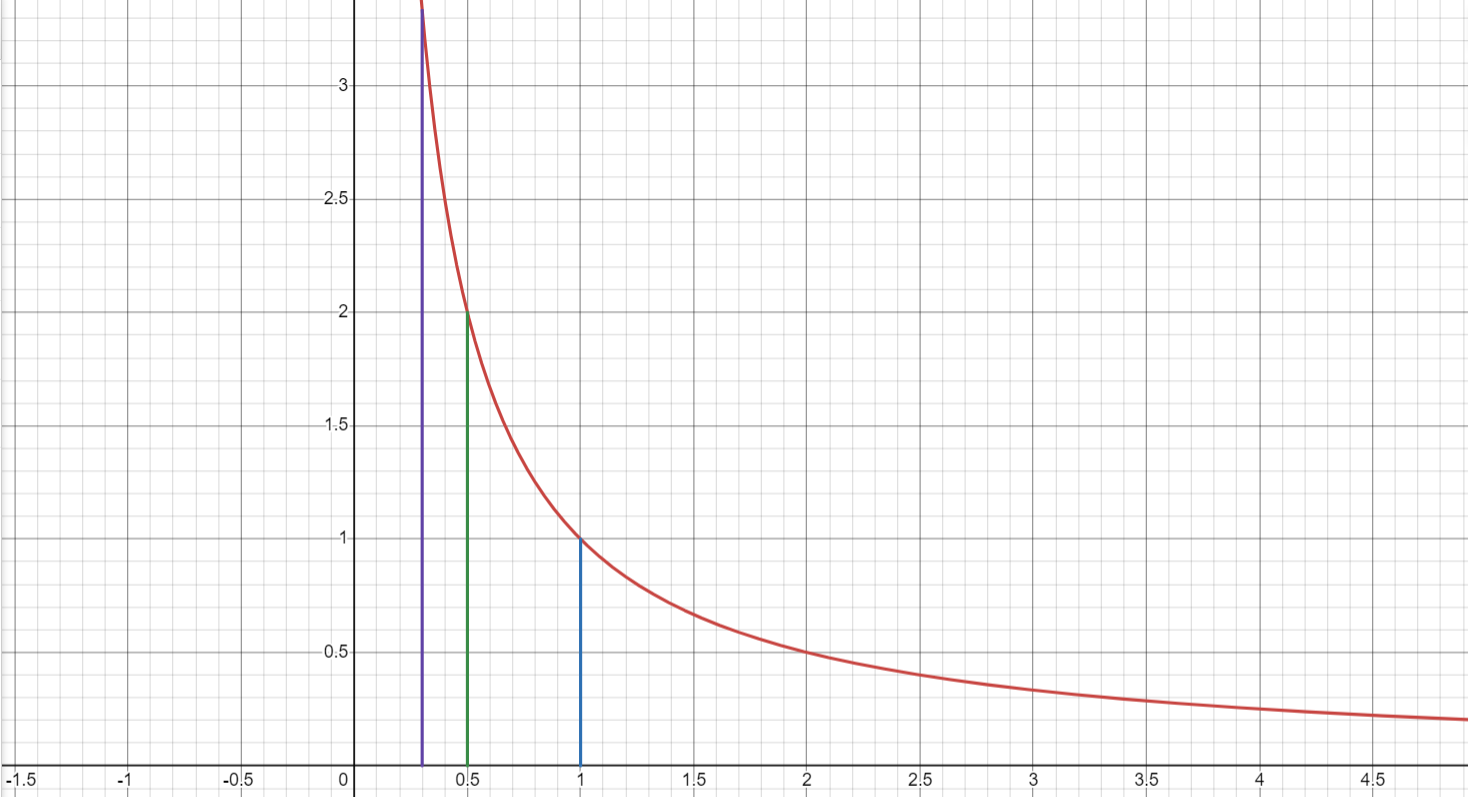
\includegraphics[width = 10cm]{pictures/improperintegral1.png}
    \centering
    \caption{Graph of $\frac{1}{x}$}
\end{figure}
Since we know that $f(x) = \frac{1}{x}$ is not defined at $x=0$, we need to use some clever trick to calculate this integral.

Let's rewrite the lower bound as $a$:
\[
    \int_a^1\frac{1}{x}\mathrm{d}x
\]
where $a>0$.

\newpage
However this integral is not equal to the original integral we want to find, since the lower bound is not equal,
but if we take the limit as $a\to 0$, this integral will approach the integral we want to find, then we can apply the fundamental theorem of calculus and find the result:
\[
    \begin{split}
        \lim_{a\to 0^-} \int_{a}^{1}\frac{1}{x}\mathrm{d}x &= \lim_{a\to 0^-}\ln a - \ln 1 \\
        & = \infty - 0 \\
        & = \infty
    \end{split}
\]
Hence we can see that this integral diverges (the limit goes to infinity).

Let's take a look at where the integral converges:
\[
    \int_0^1\frac{1}{\sqrt{x}}\mathrm{d}x
\]
We can apply the same trick we used:
\[
    \begin{split}
        \lim_{a\to 0^-} \int_{a}^{1}\frac{1}{\sqrt{x}}\mathrm{d}x &= \lim_{a\to 0^-} -2\sqrt{a} + 2\sqrt{1} \\
        & = 0 + 2 \\
        & = 2
    \end{split}
\]
Which means this integral converges (the limit has a finite value)

\subsection{Infinite Integration Bound}
We will use some example to illustrate the idea of integrating on a infinte bound:
\[
    \int_{1}^{\infty} \frac{1}{x}\mathrm{d}x
\]
Let's first replace the upper bound to $b$, and note when $b$ become very large, the integral will get very close to the original integral:
\[
    \begin{split}
        \int_{1}^{\infty} \frac{1}{x}\mathrm{d}x & = \lim_{b\to \infty} \int_{1}^{b} \frac{1}{x}\mathrm{d}x\\
        & = \lim_{b\to \infty} \ln b - \ln 1 \\
        & = \infty - 0\\
        & = \infty
    \end{split}
\]

Which means this integral diverges, we can see that there is no difference between this improper integral and the one listed above, it is both taking a limit, the same also apply for negative infinity,
the lower bound will approach negative infinity.

Let's see a integral that converges:
\[
    \int_{1}^{\infty} \frac{1}{x^2}\mathrm{d}x
\]
\[
    \begin{split}
        \int_{1}^{\infty} \frac{1}{x^2}\mathrm{d}x & = \lim_{b\to \infty} \int_{0}^{b}\frac{1}{x^2}\mathrm{d}x\\
        & = \lim_{b\to \infty} -\frac{1}{b} + 1 \\
        & = 1
    \end{split}
\]

\subsection{Both Infinite Discontinuity and Infinite Integration Bound}
There are other improper integral that can be seen as a combination of both case 1 and case 2,
but first, lets take a look at this theorem
\[
    \text{Let} \int_{a}^{b} f(x)\mathrm{d}x \text{ be an improper integral, } 
    \text{the integral only converges if } \int_{a}^{c} f(x)\mathrm{d}x \text{ and } \int_{c}^{b} f(x)\mathrm{d}x \text{ both converges}
\]
This gives a method to calculate some other improper integrals:
\[
    \int_{-\infty}^{\infty} \frac{1}{1+x^2}\mathrm{d}x
\]
We can rewrite the integral as:
\[
    \begin{split}
        \int_{-\infty}^{\infty} \frac{1}{1+x^2}\mathrm{d}x & = \int_{-\infty}^{0} \frac{1}{1+x^2}\mathrm{d}x + \int_{0}^{\infty} \frac{1}{1+x^2} \mathrm{d}x \\
        & = \lim_{b\to -\infty} \int_{b}^{0} \frac{1}{1+x^2}\mathrm{d}x + \lim_{a\to \infty} \int_{0}^{a}\frac{1}{1+x^2}\mathrm{d}x\\
        & = \arctan 0 - \lim_{b\to -\infty} \arctan b + \arctan 0 - \lim_{a\to \infty} \arctan a \\
        & = -\frac{-\pi}{2} + \frac{\pi}{2} \\
        & = \pi
    \end{split}
\]
Which means this integral converges to $\pi$.

\[
    \int_{0}^{\infty} \frac{1}{x^2}\mathrm{d}x
\]
It is convenient to split this integral into two parts and analyze them separately:
\[
    \begin{split}
        \int_{0}^{\infty} \frac{1}{x^2}\mathrm{d}x &= \int_{0}^{1}\frac{1}{x^2}\mathrm{d}x + \int_{1}^{\infty}\frac{1}{x^2} \mathrm{d}x\\
        & = \lim_{b\to 0^+} \int_{b}^{1} \frac{1}{x^2}\mathrm{d}x + \lim_{a\to \infty} \int_{1}^{a} \frac{1}{x^2} \mathrm{d}x \\
        & = -\frac{1}{1} + \lim_{b\to 0^+} \frac{1}{b} + 1\\
        & = \infty
    \end{split}
\]

There is a quicker way to do this:
\[
    \begin{split}
        \int_{0}^{1}\frac{1}{x^2}\mathrm{d}x & = -\frac{1}{1} + \lim_{b\to 0^+} \frac{1}{b} \\
        & = -1 + \infty \\
        & = \infty \\
    \end{split}
\]
This integral diverges, which by the theorem introduce earlier, the entire integral diverges.

Pretty much all improper integral can be split like this and examine separately to see if they converge or diverge.
\end{document}